\documentclass{beamer}

\beamertemplatenavigationsymbolsempty

\mode<presentation>
{
  \usetheme{default}
}

\usepackage[english]{babel}
\usepackage[latin1]{inputenc}
\usepackage{bussproofs}
\usepackage[retainorgcmds]{IEEEtrantools}

% needs debian package texlive-math-extra
\usepackage{stmaryrd} % for \llbracket, \rrbracket

\usepackage{times}
\usepackage[T1]{fontenc}
% Or whatever. Note that the encoding and the font should match. If T1
% does not look nice, try deleting the line with the fontenc.

\usepackage{tikz}
\usetikzlibrary{positioning}
\usetikzlibrary{calc}
\usetikzlibrary{matrix}

\title
{A Domain for the\\
Coinductive~Natural~Numbers\\
Part 2}

\author
{Markus~Klinik}

\institute[Radboud University Nijmegen] % (optional, but mostly needed)
{
  Radboud University Nijmegen
}

\date
{MFoCS Research Seminar 2012}


\newcommand{\arr}{\rightarrow}
\newcommand{\Arr}{\Rightarrow}
\newcommand{\semantics}[1]{\llbracket #1 \rrbracket}
\newcommand{\semanticsFd}[1]{\semantics{#1}_{F\delta}}

\begin{document}

\begin{frame}
  \titlepage
\end{frame}

\begin{frame}{Outline}
  \tableofcontents
\end{frame}

\section{A fixed point for $1+X+X$}

\subsection{Fixed points of functors}

\begin{frame}{Fixed Points of Functors}

\begin{itemize}[<+->]
  \item $\mathbf{Set}$-Functors take sets to sets
  \item Identity, powerset, cartesian product, function space
  \item Fixed point: $f(x) = x$
  \item Two sets are the same if \ldots
  \item We are interested in isomorphic sets:
      $X \sim FX$
\end{itemize}

\end{frame}


\begin{frame}{Examples}

\begin{itemize}[<+->]
  \item Cantor: $X \nsim PX$
  \item What about $1 \dot\cup X$?
\end{itemize}

\end{frame}


\begin{frame}{$\mathbb{N}$?}

Let's try $X = \mathbb{N}$

\begin{center}

$\{1,\ 2,\ 3,\ 4,\ \ldots \}$

\bigskip

$\{\langle 0, * \rangle
,\ \langle 1, 1 \rangle
,\ \langle 1, 2 \rangle
,\ \langle 1, 3 \rangle
,\ \ldots
\}$

\end{center}

\end{frame}


\newcommand{\picCpo}[1]{
\node (bottom#1) {$\bot_{#1}$};
\node (top) [above=of bottom#1] {};
\node (topleft) [left=5mm of top] {};
\node (topright) [right=5mm of top] {};
\draw (bottom#1) -- (topleft.center) -- (topright.center) -- (bottom#1);
}


\begin{frame}{The Coinductive Natural Numbers}

\begin{itemize}[<+->]

  \item We are not in $\mathbf{Set}$, we are in $\mathbf{Cpo}$
  \item Our sets have structure that functors must preserve
  \item Here: $(X, \sqsubseteq)$ where
    \begin{itemize}
      \item $\sqsubseteq$ is a partial ordering
      \item $\sqsubseteq$ is chain-complete
      \item $(X, \sqsubseteq)$ has a least element
    \end{itemize}

\end{itemize}

\onslide<+->

\begin{center}
\begin{tikzpicture}
\picCpo{}
\end{tikzpicture}
\end{center}

\end{frame}


\begin{frame}{The Separated Sum Functor}

\begin{center}
\begin{tikzpicture}

  \onslide<+->

  \picCpo{X}

  \begin{scope}[xshift=2.5cm]
  \picCpo{Y}
  \end{scope}

  \onslide<+->

  \path (1.25, -1) node (newBottom) {$\bot_{XY}$};
  \draw (bottomX) -- (newBottom) -- (bottomY);

  \onslide<+->

  \begin{scope}[xshift=5cm]
  \picCpo{Z}
  \end{scope}

  \onslide<+->

  \path (2.5, -2.3) node (newNewBottom) {$\bot_{XYZ}$};
  \draw (newBottom) -- (newNewBottom) -- (bottomZ);

\end{tikzpicture}
\end{center}

\end{frame}


\subsection{The i-place separated-sum functor}

\begin{frame}{The I-Place Separated-Sum Functor}

\onslide<+->

\begin{equation}
\sum_{i \in I}{X_i} =
  \bigcup_{i \in I} \{ \langle i, a \rangle | a \in X_i \}
  \cup \{ \bot \} \nonumber
\end{equation}

\begin{equation*}
( \sum_{i \in I}f_i ) (x) = \left\{
  \begin{array}{rl}
     \langle i, f(a) \rangle & \text{if } x = \langle i, a \rangle
                               \text{ for some } i \in I \\
    \bot                     & \text{if } x = \bot
  \end{array} \right.
\end{equation*}

\bigskip

\onslide<+->

Notation: instead of $\langle i, a \rangle$ we write $\kappa_i(a)$

\end{frame}


\begin{frame}{$1+X+X$}

\begin{equation*}
FX = \sum{(1, X, X)}
\end{equation*}

\begin{equation*}
Ff = \sum{(id, f, f)}
\end{equation*}

\end{frame}


\begin{frame}{Example}

\onslide<+->
\begin{IEEEeqnarray*}{rCl}
f & : & X \arr Y \\
Ff & : & \sum{(1, X, X)} \arr \sum{(1, Y, Y)}
\end{IEEEeqnarray*}
\onslide<+->
\begin{IEEEeqnarray*}{rCl}
Ff(\kappa_0(*)) & = & \kappa_0(id(*)) = \kappa_0(*) \\
\onslide<+->
Ff(\kappa_1(x)) & = & \kappa_1(f(x))
\end{IEEEeqnarray*}

\end{frame}


\subsection{A fixed point}

\begin{frame}{A Fixed Point for $1+X+X$}

\onslide<+->

Define $Z$: all finite and infinite words generated by
\begin{IEEEeqnarray*}{c}
Z ::= \bot\ |\ 0\ |\ S Z\ |\ \_ Z
\end{IEEEeqnarray*}

\onslide<+->

\begin{IEEEeqnarray*}{c}
  \{ \bot,\ 0,\ S\bot,\ S0,\ \_\bot,\ \_0,\
     S\_\bot,\ S\_0,\ \_S\bot,\ \_S0,\ \ldots
  \}
\end{IEEEeqnarray*}

\end{frame}


\begin{frame}{Is Z a Fixed Point For $1+X+X$?}

\begin{columns}[totalwidth=.7\textwidth]

  \begin{column}{.5\textwidth}
  \begin{IEEEeqnarray*}{rCl}
  \IEEEeqnarraymulticol{3}{c}{\delta : Z \arr FZ}
  \\
  \delta(\bot) & = & \bot
  \\
  \delta(0) & = & \kappa_0(*)
  \\
  \delta(Sw) & = & \kappa_1(w)
  \\
  \delta(\_w) & = & \kappa_2(w)
  \end{IEEEeqnarray*}
  \end{column}

  \begin{column}{.5\textwidth}
  \begin{IEEEeqnarray*}{rCl}
  \IEEEeqnarraymulticol{3}{c}{\delta' : FZ \arr Z}
  \\
  \delta'(\bot) & = & \bot
  \\
  \delta'(\kappa_0(*)) & = & 0
  \\
  \delta'(\kappa_1(w)) & = & Sw
  \\
  \delta'(\kappa_2(w)) & = & \_w
  \end{IEEEeqnarray*}
  \end{column}

\end{columns}

\end{frame}

\begin{frame}[fragile]{Is Z The Largest Fixed Point?}

\begin{itemize}

  \item Coalgebras $(C, \gamma : C \arr FC)$
  \item Final coalgebra $(Z, \delta)$
  \begin{itemize}
    \item Existence
    \item Unicity
  \end{itemize}

\end{itemize}

\begin{center}
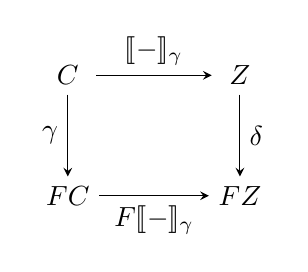
\begin{tikzpicture}
\matrix (m) [matrix of math nodes,row sep=3em,column sep=4em,minimum width=2em]
  {
     C & Z \\
     FC & FZ \\
  };
  \path[-stealth]
    (m-1-1) edge node [left] {$\gamma$} (m-2-1)
            edge node [above] {$\semantics{-}_{\gamma}$} (m-1-2)
    (m-2-1.east|-m-2-2) edge node [below] {$F\semantics{-}_{\gamma}$} (m-2-2)
    (m-1-2) edge node [right] {$\delta$} (m-2-2);
\end{tikzpicture}
\end{center}

\end{frame}


\begin{frame}{Existence}

Define $\semantics{-}$ and prove
  $\delta \circ \semantics{-} = F\semantics{-} \circ \gamma$.

\begin{IEEEeqnarray*}{rCl}
\semantics{a} & = & \text{ case } \gamma(a) \text{ of}
\\
\bot_C & = & \bot_Z
\\
\kappa_0(*) & = & 0
\\
\kappa_1(b) & = & S \semantics{b}
\\
\kappa_2(b) & = & \_ \semantics{b}
\end{IEEEeqnarray*}

\end{frame}


\begin{frame}[fragile]{Unicity}

For any other $f : C \arr Z$ which makes the diagram commute:

\begin{equation*}
  f = \semantics{-}
\end{equation*}

\begin{center}
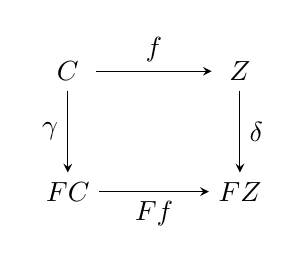
\begin{tikzpicture}
\matrix (m) [matrix of math nodes,row sep=3em,column sep=4em,minimum width=2em]
  {
     C & Z \\
     FC & FZ \\
  };
  \path[-stealth]
    (m-1-1) edge node [left] {$\gamma$} (m-2-1)
            edge node [above] {$f$} (m-1-2)
    (m-2-1.east|-m-2-2) edge node [below] {$Ff$} (m-2-2)
    (m-1-2) edge node [right] {$\delta$} (m-2-2);
\end{tikzpicture}
\end{center}

\end{frame}


\begin{frame}{First Try}

\onslide<1->

\begin{itemize}
  \item
    \alt<1>{Want: $f(a) = \semantics{a}, \forall a \in C$}
    {Also okay: $\delta(f(a)) = \delta(\semantics{a}), \forall a \in C$}
  \item Have: two commutative diagrams
\end{itemize}

\onslide<4->{$\gamma(a) = \kappa_1(b)$}

\onslide<6->{$\delta(Sw) = \kappa_1(w)$}
\begin{IEEEeqnarray*}{CCCCCCCCC}
\onslide<2->
\delta(f(a))
\onslide<3->
   & = & Ff(\gamma(a))
\onslide<4->
   & = & Ff(\kappa_1(b))
\onslide<5->
   & = & \kappa_1(f(b))
\onslide<6->
   & = & \delta(Sf(b)) \\
\onslide<2->
\delta(\semantics{a})
\onslide<3->
   & = & F\semantics{-}(\gamma(a))
\onslide<4->
   & = & F\semantics-(\kappa_1(b))
\onslide<5->
   & = & \kappa_1(\semantics{b})
\onslide<6->
   & = & \delta(S\semantics{b})
\end{IEEEeqnarray*}

\end{frame}


\begin{frame}{Coinduction FTW!}

We need a proof by bisimulation

\begin{IEEEeqnarray*}{c}
R \subseteq FZ \times FZ =
  \{ \langle \delta(wf(a)) , \delta(w\semantics{a}) \rangle
   \ |\  a \in C, w \in \{ S, \_ \}^*
  \}
\end{IEEEeqnarray*}

\end{frame}


\begin{frame}[fragile]{Let's Try}

Have: $R =
  \{ \langle \delta(wf(a)) , \delta(w\semantics{a}) \rangle
   \ |\  a \in C, w \in \{ S, \_ \}^*
  \}$

\onslide<2->{$w = Sw'$}
\begin{IEEEeqnarray*}{CCCCCCC}
\delta(wf(a))
 \onslide<2->
 & = & \delta(Sw'f(a))
 \onslide<3->
 & = & \kappa_1(w'f(a))
 \onslide<4->
 & = & \kappa_1(\textcolor{red}{\delta(}w'f(a)\textcolor{red}{)})
\\
\onslide<1->
\delta(w\semantics{a})
 \onslide<2->
 & = & \delta(Sw'\semantics{a})
 \onslide<3->
 & = & \kappa_1(w'\semantics{a})
 \onslide<4->
 & = & \kappa_1(\textcolor{red}{\delta(}w'\semantics{a}\textcolor{red}{)})
\end{IEEEeqnarray*}

\end{frame}


\begin{frame}{Lemma}

\onslide<+->

\begin{IEEEeqnarray*}{C}
  \semanticsFd{-} \circ \delta = \text{id}_{Z}
\end{IEEEeqnarray*}
\begin{IEEEeqnarray*}{C}
\onslide<+->
  \delta : Z \arr FZ
  \\
  (FZ, F\delta : FZ \arr FFZ)
  \\
  \semanticsFd{-} : FZ \arr Z
\end{IEEEeqnarray*}

\end{frame}


\begin{frame}[fragile]{Let's Try}

Have: $R =
  \{ \langle \delta(wf(a)) , \delta(w\semantics{a}) \rangle
   \ |\  a \in C, w \in \{ S, \_ \}^*
  \}$

{$w = Sw'$}
\begin{IEEEeqnarray*}{CCCCCCC}
\delta(wf(a))
 & = & \delta(Sw'f(a))
 & = & \kappa_1(w'f(a))
 & = & \kappa_1(\textcolor{red}{\llbracket\delta(}w'f(a)\textcolor{red}{)\rrbracket_{F\delta}})
\\
\delta(w\semantics{a})
 & = & \delta(Sw'\semantics{a})
 & = & \kappa_1(w'\semantics{a})
 & = & \kappa_1(\textcolor{red}{\llbracket\delta(}w'\semantics{a}\textcolor{red}{)\rrbracket_{F\delta}})
\end{IEEEeqnarray*}

\end{frame}


\begin{frame}{Intermission}

Done:

\begin{itemize}
  \item $F$ is a handy variant of disjoint union
  \item $Z$ is a fixed point of $F$
  \item $Z$ is the largest fixed point of $F$
\end{itemize}

To do:

\begin{itemize}
  \item $Z$ is a domain
  \item $Z$ somehow \emph{is} the lazy natural numbers
\end{itemize}

\end{frame}


\section{A domain for $1+X+X$}

\subsection{The domain}

\begin{frame}{The Domain of Z}

Let the relation $\sqsubset$ on $Z \times Z$ be defined as: two
words $s$ and $t$ are in relation $s \sqsubset t$ iff $s$ is finite and $|s|
\leq |t|$ and $s_{|s|-1} = \bot$ and for all $i < |s|-1: s_i = t_i$.

\bigskip

Let $\sqsubseteq$ be the reflexive closure of $\sqsubset$.

\end{frame}


\begin{frame}{The Domain of Z}

\begin{center}
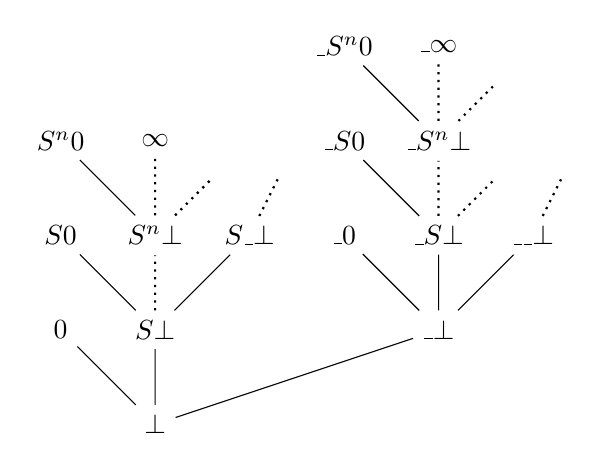
\begin{tikzpicture}
 [ grow'=up
 , scale=1.2
 , level distance=1cm
 , level 1/.style={sibling distance=3cm}
 , level 2/.style={sibling distance=1cm}
 , normal/.style={thin, solid}
 , skipping/.style={thick, dotted}
 , and so on/.style={thick, dotted, sibling distance=0.6cm, level distance=0.6cm}
 ]
  \node {$\bot$}
    child [sibling distance=1cm] { node {$0$} }
    child
    {
      node {$S\bot$}
      child { node {$S0$} }
      child [skipping]
      {
        %node {$SS\bot$}
        %child { node {$SS0$} }
        %child [skipping]
        %{
          node {$S^n\bot$}
          child [normal] { node {$S^n0$} }
          child [skipping] { node {$\infty$} }
          child [and so on] {}
        %}
        %child [and so on] {}
      }
      child
      {
        node {$S\_\bot$}
        child [missing] {}
        child [and so on] {}
      }
    }
    child
    {
      node {$\_ \bot$}
      child { node {$\_0$} }
      child
      {
        node {$\_S\bot$}
        child { node {$\_S0$} }
        child [skipping]
        {
          node {$\_S^n\bot$}
          child [normal] { node {$\_S^n0$} }
          child { node {$\_\infty$} }
          child [and so on] {}
        }
        child [and so on] {}
      }
      child
      {
        node {$\_\_\bot$}
        child [missing] {}
        %child [missing] {}
        child [and so on] {}
      }
    }
  ;
\end{tikzpicture}
\end{center}

\end{frame}


\subsection{Its relation to $1+X$}

\begin{frame}{Projection from $1+X+X$ to $1+X$}

\onslide<+->

\begin{columns}

\begin{column}{.5\textwidth}
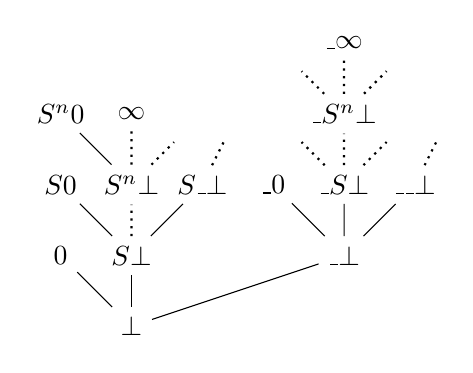
\begin{tikzpicture}
 [ grow'=up
 , scale=0.9
 , level distance=1cm
 , level 1/.style={sibling distance=3cm}
 , level 2/.style={sibling distance=1cm}
 , normal/.style={thin, solid}
 , skipping/.style={thick, dotted}
 , and so on/.style={thick, dotted, sibling distance=0.6cm, level distance=0.6cm}
 ]
  \node {$\bot$}
    child [sibling distance=1cm] { node {$0$} }
    child
    {
      node {$S\bot$}
      child { node {$S0$} }
      child [skipping]
      {
        %node {$SS\bot$}
        %child { node {$SS0$} }
        %child [skipping]
        %{
          node {$S^n\bot$}
          child [normal] { node {$S^n0$} }
          child [skipping] { node {$\infty$} }
          child [and so on] {}
        %}
        %child [and so on] {}
      }
      child
      {
        node {$S\_\bot$}
        child [missing] {}
        child [and so on] {}
      }
    }
    child
    {
      node {$\_ \bot$}
      child { node {$\_0$} }
      child
      {
        node {$\_S\bot$}
        child [and so on]
        child [skipping]
        {
          node {$\_S^n\bot$}
          child [and so on] {}
          child { node {$\_\infty$} }
          child [and so on] {}
        }
        child [and so on] {}
      }
      child
      {
        node {$\_\_\bot$}
        child [missing] {}
        %child [missing] {}
        child [and so on] {}
      }
    }
  ;
\end{tikzpicture}
\end{column}

\begin{column}{.5\textwidth}
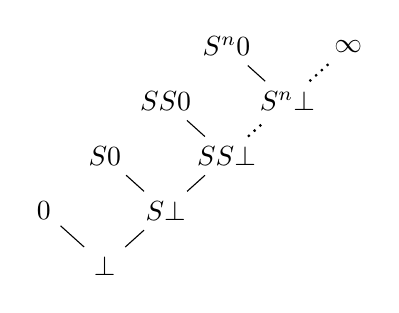
\begin{tikzpicture}[scale=1.1]
  \node {$\bot$} [grow'=up, sibling distance=4.0em, level distance=1.8em]
    child { node {$0$} }
    child
    {
      node {$S\bot$}
      child { node {$S0$} }
      child
      {
        node {$SS\bot$}
        child { node {$SS0$} }
        child [thick, dotted]
        {
          node {$S^n\bot$}
          child [thin, solid] { node {$S^n0$} }
          child { node {$\infty$} }
        }
      }
    }
  ;
\end{tikzpicture}
\end{column}

\end{columns}

\onslide<+->

\begin{IEEEeqnarray}{rCl}
p(z) & = & \bot
\\
p(Sw') & = & Sp(w')
\\
p(\_w') & = & p(w')
\\
p(0) & = & 0 \nonumber
\\
p(\bot) & = & \bot \nonumber
\end{IEEEeqnarray}

\end{frame}


\begin{frame}{Questions}
\end{frame}


\end{document}
